% CMU-themed Beamer Presentation
\documentclass[aspectratio=169,12pt]{beamer}

% CMU Theme Setup
\usetheme{Madrid}
\usecolortheme{default}

% CMU Colors
\definecolor{CMURed}{RGB}{196,18,48}
\definecolor{CMUGray}{RGB}{102,102,102}
\definecolor{CMULightGray}{RGB}{214,210,196}

\setbeamercolor{structure}{fg=CMURed}
\setbeamercolor{palette primary}{bg=CMURed,fg=white}
\setbeamercolor{palette secondary}{bg=CMUGray,fg=white}
\setbeamercolor{palette tertiary}{bg=CMURed,fg=white}
\setbeamercolor{palette quaternary}{bg=CMUGray,fg=white}
\setbeamercolor{titlelike}{parent=palette primary}
\setbeamercolor{block title}{bg=CMURed,fg=white}
\setbeamercolor{block body}{bg=CMULightGray,fg=black}
\setbeamercolor{frametitle}{bg=CMURed,fg=white}

% Packages
\usepackage{graphicx}
\usepackage{booktabs}
\usepackage{listings}
\usepackage{amsmath}
\usepackage{amssymb}
\usepackage{hyperref}
\usepackage{tikz}
\usetikzlibrary{shapes,arrows,positioning,calc}
\usepackage{pifont}
\newcommand{\cmark}{\ding{51}}%
\newcommand{\xmark}{\ding{55}}%

% Code listing style
\lstset{
  basicstyle=\ttfamily\small,
  breaklines=true,
  frame=single,
  language=Python,
  showstringspaces=false,
  commentstyle=\color{CMUGray},
  keywordstyle=\color{CMURed},
  backgroundcolor=\color{CMULightGray}
}

% Title information
\title[RL for Triton Optimization]{Beyond TritonRL: Reinforcement Learning for Triton Kernel Optimization with Modular Extensions}
\author{Vanshaj Agrawal}
\institute{Carnegie Mellon University}
\date{December 15, 2025}

\begin{document}

% Title slide
\begin{frame}
\titlepage
\end{frame}

% Introduction & Motivation
\begin{frame}{Introduction \& Motivation}
\framesubtitle{Why This Matters}

\begin{block}{The Problem}
\begin{itemize}
    \item \textbf{ML system performance} critically depends on efficient GPU kernels
    \item \textbf{Triton}: Python DSL for GPU programming (easier than CUDA)
    \item \textbf{Challenge}: Generating optimal Triton code is hard
    \item \textbf{Kernel fusion} (combining operations) is especially challenging
\end{itemize}
\end{block}

\vspace{0.3cm}

\begin{block}{Current State: TritonRL}
\begin{itemize}
    \item Uses RL to improve kernel generation
    \item \textcolor{CMURed}{\textbf{Only 7\% correctness}} on complex fusion tasks (Level 2)
    \item 63\% on basic operations (Level 1)
\end{itemize}
\end{block}

\vspace{0.3cm}
\centering
\Large \textbf{Can we do better with targeted extensions?}
\end{frame}

% Problem Statement
\begin{frame}{Problem Statement}

\begin{columns}[T]
\column{0.48\textwidth}
\textbf{Research Questions:}
\begin{enumerate}
    \item Can \textcolor{CMURed}{multi-input testing} improve generalization?
    \item Does \textcolor{CMURed}{staged evaluation} improve training efficiency?
    \item Can \textcolor{CMURed}{adaptive curriculum} help with complex fusion?
    \item Does \textcolor{CMURed}{timing calibration} reduce noise?
\end{enumerate}

\column{0.48\textwidth}
\textbf{Task Definition:}
\begin{itemize}
    \item \textbf{Input}: Natural language description + PyTorch reference
    \item \textbf{Output}: Correct \& performant Triton kernel
\end{itemize}

\vspace{0.3cm}
\textbf{Challenge: Level 2 Fusion}
\begin{itemize}
    \item Fused GEMM+bias
    \item Conv+BatchNorm+ReLU
    \item Multiple operations combined correctly
\end{itemize}
\end{columns}

\end{frame}

% Related Work
\begin{frame}{Related Work}

\begin{columns}[T]
\column{0.48\textwidth}
\textbf{Prior Approaches:}
\begin{itemize}
    \item TVM/Ansor: Search-based
    \item AlphaCode: RL for code
    \item Curriculum Learning
\end{itemize}

\vspace{0.3cm}
\textbf{TritonRL Baseline:}
\begin{itemize}
    \item SFT + RL (best-of-N)
    \item N=10, keeps K=3
    \item \textcolor{CMURed}{\textbf{Limits}}: Fragile verification
\end{itemize}

\column{0.48\textwidth}
\textbf{Our Improvements:}
\begin{enumerate}
    \item Multi-input testing
    \item Staged evaluation
    \item Adaptive curriculum
    \item Calibrated timing
\end{enumerate}

\vspace{0.3cm}
All extensions are \textbf{modular} and independently toggleable

\end{columns}

\end{frame}

% System Architecture Overview
\begin{frame}{System Architecture Overview}

\begin{center}
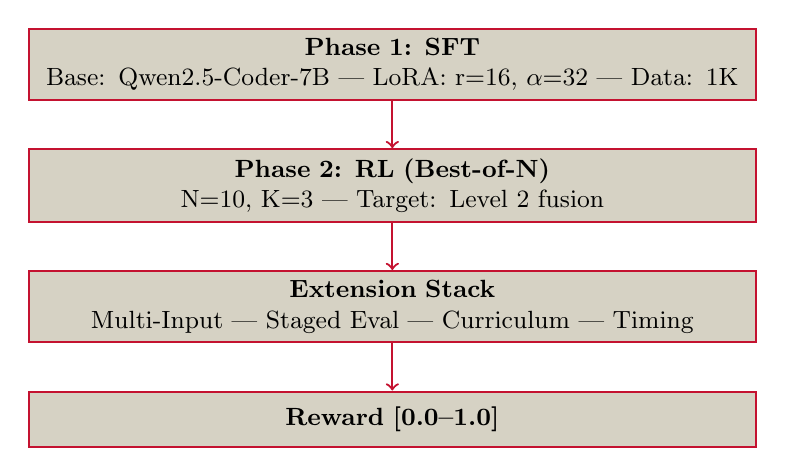
\begin{tikzpicture}[
    node distance=0.6cm,
    box/.style={rectangle, draw=CMURed, thick, fill=CMULightGray,
                text width=9cm, align=center, minimum height=0.7cm, font=\small},
    arrow/.style={->, thick, CMURed}
]

\node[box] (sft) {\textbf{Phase 1: SFT}\\
Base: Qwen2.5-Coder-7B | LoRA: r=16, $\alpha$=32 | Data: 1K};

\node[box, below=of sft] (rl) {\textbf{Phase 2: RL (Best-of-N)}\\
N=10, K=3 | Target: Level 2 fusion};

\node[box, below=of rl] (ext) {\textbf{Extension Stack}\\
Multi-Input | Staged Eval | Curriculum | Timing};

\node[box, below=of ext] (reward) {\textbf{Reward [0.0--1.0]}};

\draw[arrow] (sft) -- (rl);
\draw[arrow] (rl) -- (ext);
\draw[arrow] (ext) -- (reward);

\end{tikzpicture}
\end{center}

\vspace{0.2cm}
\centering
\textbf{Key Design}: Modular, independently toggleable extensions

\end{frame}

% Component Architecture
\begin{frame}{System Design: Component Architecture}

\begin{center}
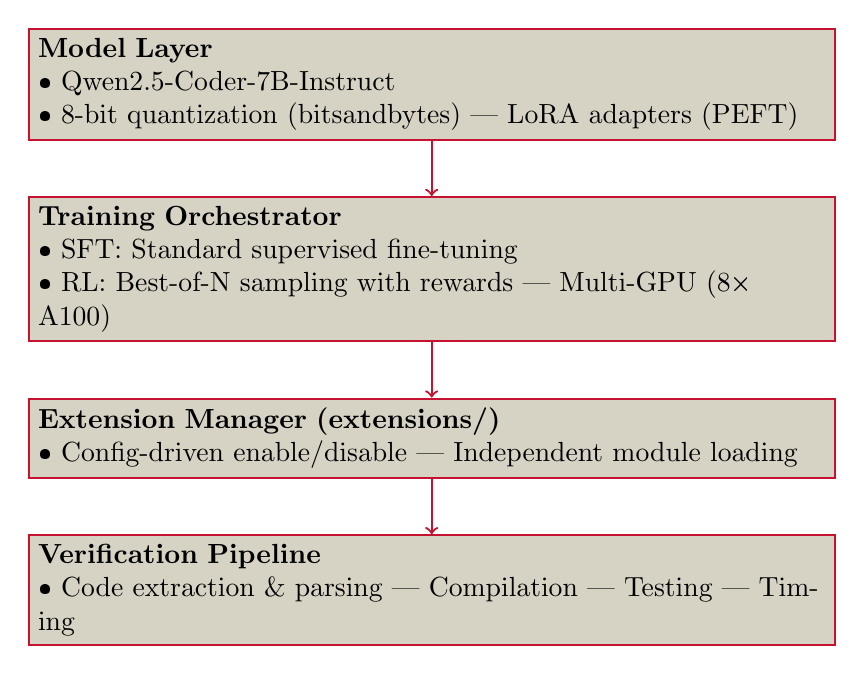
\begin{tikzpicture}[
    node distance=0.7cm,
    box/.style={rectangle, draw=CMURed, thick, fill=CMULightGray,
                text width=10cm, align=left, minimum height=1cm},
    arrow/.style={->, thick, CMURed}
]

\node[box] (model) {\textbf{Model Layer}\\
• Qwen2.5-Coder-7B-Instruct\\
• 8-bit quantization (bitsandbytes) | LoRA adapters (PEFT)};

\node[box, below=of model] (train) {\textbf{Training Orchestrator}\\
• SFT: Standard supervised fine-tuning\\
• RL: Best-of-N sampling with rewards | Multi-GPU (8× A100)};

\node[box, below=of train] (extman) {\textbf{Extension Manager (extensions/)}\\
• Config-driven enable/disable | Independent module loading};

\node[box, below=of extman] (verify) {\textbf{Verification Pipeline}\\
• Code extraction \& parsing | Compilation | Testing | Timing};

\draw[arrow] (model) -- (train);
\draw[arrow] (train) -- (extman);
\draw[arrow] (extman) -- (verify);

\end{tikzpicture}
\end{center}

\end{frame}

% Data Flow
\begin{frame}[fragile]{System Design: Data Flow}

\begin{block}{Training Loop Flow}
\small
\begin{enumerate}
    \item \textbf{Sample Task}
    \begin{itemize}
        \item Level 1: Basic kernels (matmul, softmax)
        \item Level 2: Fusion tasks (GEMM+bias+ReLU)
    \end{itemize}

    \item \textbf{Generate N=10 Candidates}
    \begin{itemize}
        \item Model inference with sampling
        \item Temperature-controlled diversity
    \end{itemize}

    \item \textbf{Extension Stack Processing}
    \begin{itemize}
        \item Multi-Input: 5 test cases
        \item Staged Eval: 5-stage filtering
        \item Curriculum: Sample by level
        \item Timing: Calibrated measurement
    \end{itemize}

    \item \textbf{Compute Rewards [0.0--1.0]}
    \begin{itemize}
        \item Correctness: 0.0 or 0.7
        \item Performance: 0.0 to 0.3 bonus
        \item Partial credit for stages
    \end{itemize}

    \item \textbf{Select Top K=3 Candidates} → Update model via RL
\end{enumerate}
\end{block}

\end{frame}

% Extension Module Interface
\begin{frame}[fragile]{System Design: Extension Module Interface}

\begin{block}{Modular Design Pattern}
\begin{lstlisting}
# Base interface all extensions implement
class Extension:
    def __init__(self, config):
        self.enabled = config.get('enabled', False)

    def process(self, candidate, task):
        if not self.enabled:
            return candidate  # Pass-through
        return self._apply(candidate, task)

# Extensions stack independently
extensions = [
    MultiInputTesting(config),
    StagedEvaluation(config),
    AdaptiveCurriculum(config),
    CalibratedTiming(config)
]

for ext in extensions:
    candidate = ext.process(candidate, task)
\end{lstlisting}
\end{block}

\textbf{Benefits:} Toggle independently • Easy to extend • Clean separation

\end{frame}

% Implementation Stack
\begin{frame}{System Design: Implementation Stack}

\begin{table}
\small
\begin{tabular}{lll}
\toprule
\textbf{Layer} & \textbf{Technology} & \textbf{Rationale} \\
\midrule
Model & Qwen2.5-Coder-7B & SOTA code generation \\
Fine-tuning & LoRA (PEFT) & Memory-efficient training \\
Quantization & 8-bit (bitsandbytes) & Fit on 40GB A100s \\
Framework & PyTorch + Transformers & Industry standard \\
Kernel DSL & Triton 2.1+ & Target language \\
Distributed & Accelerate & Multi-GPU coordination \\
\bottomrule
\end{tabular}
\end{table}

\vspace{0.3cm}

\begin{columns}[T]
\column{0.48\textwidth}
\textbf{File Organization:}
\small
\begin{itemize}
    \item \texttt{extensions/}: 4 modules
    \item \texttt{src/}: Training scripts
    \item \texttt{configs/}: YAML configs
    \item \texttt{data/}: KernelBook dataset
\end{itemize}

\column{0.48\textwidth}
\textbf{Hardware:}
\small
\begin{itemize}
    \item SFT: 8× A100 40GB
    \item RL: 1× A10G 24GB
    \item 8-bit quantization: ~7GB
    \item LoRA: 0.5\% parameters
\end{itemize}
\end{columns}

\end{frame}

% Extension 1
\begin{frame}{Extension 1: Multi-Input Testing}

\begin{block}{Problem}
Single test case → models overfit to specific patterns
\end{block}

\begin{block}{Solution: Generate 5 Diverse Test Inputs}
\begin{enumerate}
    \item Original input
    \item Scaled values (×2.0)
    \item Different random seed
    \item Larger dimensions
    \item Different precision
\end{enumerate}
\end{block}

\begin{alertblock}{Benefit}
Catches edge cases that single input misses
\end{alertblock}

\end{frame}

% Extension 2
\begin{frame}{Extension 2: Staged Evaluation}

\begin{block}{Problem}
Evaluating all generated kernels wastes compute
\end{block}

\begin{block}{Solution: 5-Stage Funnel}
\begin{table}
\small
\begin{tabular}{llll}
\toprule
\textbf{Stage} & \textbf{Check} & \textbf{Time} & \textbf{Reward on Fail} \\
\midrule
1 & AST syntax & ms & 0.0 \\
2 & Compilation & sec & 0.3 \\
3 & Tiny run (4×4) & sec & 0.5 \\
4 & Full run & sec & 0.7 \\
5 & Timing & min & 1.0 \\
\bottomrule
\end{tabular}
\end{table}
\end{block}

\begin{alertblock}{Benefit}
\textbf{35-40\% throughput improvement} in unit tests
\end{alertblock}

\end{frame}

% Extension 3
\begin{frame}{Extension 3: Adaptive Curriculum}

\begin{block}{Problem}
Fixed task distribution forces premature training on hard tasks
\end{block}

\begin{block}{Solution: Dynamic Schedule}
\begin{itemize}
    \item \textbf{Start}: 10\% Level 2 (fusion) tasks
    \item \textbf{Increase}: Linearly to 50\% when Level 1 accuracy > 40\%
    \item \textbf{Logic}: Build solid foundations before complexity
\end{itemize}
\vspace{0.3cm}
\centering
\texttt{Level 2 \% = 0.1 + 0.4 × (L1\_accuracy / 0.4) if L1 < 0.4 else 0.5}
\end{block}

\begin{alertblock}{Benefit}
Progressive difficulty ensures model readiness
\end{alertblock}

\end{frame}

% Extension 4
\begin{frame}{Extension 4: Calibrated Timing}

\begin{block}{Problem}
Single measurements have 15\% noise from GPU scheduling
\end{block}

\begin{block}{Solution: Statistical Protocol}
\begin{enumerate}
    \item \textbf{Warmup}: 10 runs to stabilize GPU state
    \item \textbf{Measurement}: 50 trials with CUDA events
    \item \textbf{Aggregation}: Trimmed mean (remove 10\% outliers)
\end{enumerate}
\end{block}

\begin{alertblock}{Benefit}
Reduced coefficient of variation: \textbf{15\% → 5\%}
\end{alertblock}

\end{frame}

% Evaluation Setup
\begin{frame}{Evaluation Setup}

\begin{columns}[T]
\column{0.48\textwidth}
\textbf{Hardware:}
\begin{itemize}
    \item Initially: 8× A100 40GB
    \item Later: 1× A10G (budget)
\end{itemize}

\vspace{0.3cm}
\textbf{Dataset:}
\begin{itemize}
    \item Training: 1,000 samples
    \item KernelBook: 18K total
    \item Eval: 20 Level 2 fusion tasks
\end{itemize}

\column{0.48\textwidth}
\textbf{Metrics:}
\begin{itemize}
    \item Valid Rate: \% passing AST
    \item Compiled: \% compiling
    \item \textcolor{CMURed}{\textbf{Correct}}: \% with correct outputs
    \item Speedup: vs. PyTorch
\end{itemize}

\vspace{0.3cm}
\textbf{Hyperparameters:}
\begin{itemize}
    \item SFT: 1 epoch, lr=2e-4
    \item RL: N=10, K=3
    \item Curriculum: p=0.1→0.5
\end{itemize}
\end{columns}

\end{frame}

% Results
\begin{frame}{Results: Honest Reporting}

\begin{alertblock}{Training Completed Successfully}
\cmark~SFT loss: 0.757 → 0.199\\
\cmark~RL training: 10/10 tasks completed\\
\cmark~No crashes or failures
\end{alertblock}

\vspace{0.3cm}

\begin{exampleblock}{But Performance Significantly Underperformed}
\begin{table}
\begin{tabular}{lccc}
\toprule
\textbf{Task Level} & \textbf{Baseline} & \textbf{Ours (Best)} & \textbf{Diff} \\
\midrule
Level 1 (Basic) & 63\% & \textcolor{CMURed}{\textbf{15\%}} & \textcolor{CMURed}{-48\%} \\
Level 2 (Fusion) & 7\% & \textcolor{CMURed}{\textbf{3\%}} & \textcolor{CMURed}{-4\%} \\
\bottomrule
\end{tabular}
\end{table}
\end{exampleblock}

\vspace{0.3cm}
\centering
\Large \textcolor{CMURed}{\textbf{Our extensions did NOT improve over baseline}}

\end{frame}

% Why Did We Underperform
\begin{frame}{Why Did We Underperform?}

\begin{enumerate}
    \item \textbf{Evaluation Pipeline Issues}
    \begin{itemize}
        \item Initial verifier bugs (0\% valid rate)
        \item After fixes: revealed poor model performance
    \end{itemize}

    \item \textbf{Limited Training Scale}
    \begin{itemize}
        \item Used \textbf{1,000 samples} vs. full 18K dataset
        \item Only \textbf{1 SFT epoch} vs. likely more for baseline
        \item Limited RL iterations (budget constraints)
    \end{itemize}

    \item \textbf{Extension Interactions}
    \begin{itemize}
        \item Individual extensions showed promise in unit tests
        \item Combined effect may have introduced issues
        \item OR insufficient training to see benefits
    \end{itemize}

    \item \textbf{Model Selection}
    \begin{itemize}
        \item Qwen2.5-Coder-7B may not be optimal for Triton
        \item Baseline may have used different/better model
    \end{itemize}
\end{enumerate}

\end{frame}

% Lessons Learned
\begin{frame}{Lessons Learned}

\begin{block}{Integration Challenges}
\begin{enumerate}
    \item \textbf{Output format brittleness}
    \begin{itemize}
        \item LLMs generate varied formats
        \item Need robust parsing, not simple regex
    \end{itemize}

    \item \textbf{Configuration management}
    \begin{itemize}
        \item Path mismatches cause silent failures
        \item Need centralized validation
    \end{itemize}

    \item \textbf{Iterative debugging}
    \begin{itemize}
        \item RL for code generation requires multiple iterations
        \item Cloud costs make this expensive
    \end{itemize}

    \item \textbf{Verification before training}
    \begin{itemize}
        \item "Dry runs" with dummy models catch bugs early
        \item Saves expensive GPU time
    \end{itemize}
\end{enumerate}
\end{block}

\end{frame}

% Key Takeaways
\begin{frame}{Key Takeaways}

\begin{block}{1. Good Ideas $\neq$ Good Results}
Theoretically motivated extensions can fail in practice
\end{block}

\begin{block}{2. Limited Budgets Create Ambiguity}
Hard to distinguish:
\begin{itemize}
    \item "Extensions hurt performance"
    \item vs. "Insufficient training to see benefits"
\end{itemize}
\end{block}

\begin{block}{3. Negative Results Are Valuable}
\begin{itemize}
    \item Validate on small scale first
    \item Ablation studies are critical
    \item Need to isolate individual contributions
\end{itemize}
\end{block}

\begin{block}{4. Honest Reporting Matters}
Failures teach as much as successes
\end{block}

\end{frame}

% Contributions
\begin{frame}{Contributions Summary}

\begin{columns}[T]
\column{0.48\textwidth}
\begin{block}{What We Achieved \cmark}
\begin{itemize}
    \item Complete end-to-end implementation
    \item Full training pipeline (SFT + RL)
    \item Honest negative results
    \item Analysis of failures
    \item Lessons for future work
\end{itemize}
\end{block}

\column{0.48\textwidth}
\begin{alertblock}{What We Cannot Claim \xmark}
\begin{itemize}
    \item Extensions did NOT improve
    \item No ablation studies
    \item Cannot isolate root cause
    \item Unclear if extensions hurt or training insufficient
\end{itemize}
\end{alertblock}
\end{columns}

\vspace{0.5cm}

\begin{exampleblock}{Value}
Negative results are contributions • Demonstrated need for validation • Lessons for RL-based code generation research
\end{exampleblock}

\end{frame}

% Conclusion
\begin{frame}{Conclusion}

\begin{block}{Problem Addressed}
TritonRL achieves only 7\% on kernel fusion tasks
\end{block}

\begin{block}{Our Approach}
4 modular extensions targeting specific weaknesses:
Multi-input • Staged evaluation • Adaptive curriculum • Calibrated timing
\end{block}

\begin{alertblock}{Results}
Training succeeded, but \textcolor{CMURed}{\textbf{underperformed baseline}}\\
Likely due to limited data/training + possible extension issues
\end{alertblock}

\begin{exampleblock}{Key Message}
Theoretically sound extensions don't always translate to improvements.\\
Small-scale validation and ablation studies are critical before scaling up.
\end{exampleblock}

\end{frame}

% Thank You
\begin{frame}[plain]
\begin{center}
\Huge \textcolor{CMURed}{\textbf{Thank You!}}

\vspace{1.5cm}

\Large
\textbf{Code \& Resources}

\normalsize
\vspace{0.5cm}
Repository: \texttt{github.com/vanshajagrawal/beyondtritonrl}

\vspace{0.3cm}
Presentation: Google Drive

\vspace{1.5cm}

\Large
\textcolor{CMURed}{\textbf{Questions?}}
\end{center}
\end{frame}

\end{document}
